Die Massenspektrometrie besitzt vielfältige Anwendungen z. B. in der Chemie zur quantitativen und qualitativen Analyse von Substanzen, oder auch in der Industrie.
In diesem Versuch werden unter anderem die Auftrittsenergie von Argon und die Dissoziationsenergien von Stickstoff bestimmt, sowie eine quantitative und qualitative Analyse durchgeführt.

\section{Vakuumpumpsysteme}
Um das Massenspektrometer betreiben zu können, muss die mittlere freie Weglänge der Gasmoleküle größer als die Länge des Spektrometers sein. Um die erforderlichen niedrigen Drücke zu erreichen, werden in diesem Versuch zwei unterschiedliche Pumpen verwendet.
Zunächst wird mittels einer Drehschieberpumpe ein Vorvakuum ($p\approx\SI{3e-2}{\milli\bar}$) erzeugt. Schließlich wird eine Turbomolekularpumpe verwendet, um ein Hochvakuum ($p\approx\SI{e-7}{\milli\bar}$) zu erreichen.

\subsection{Drehschieberpumpe}

Eine Drehschieberpumpe (siehe Abb. \ref{fig011}) besteht aus einem Rotor, an dem Federn angebracht sind. Zu Beginn des Pumpvorgangs tritt das Gas in den Schöpfraum ein. Es wird dann von der Feder, die durch die Federkraft oder durch die Zentrifugalkraft an die Wand gepresst wird, mitgenommen und verdichtet.
Die Pumpwirkung kommt dadurch zustande, dass beim Ansaugvorgang das Schöpfvolumen erhöht wird.

\begin{figure}[tb]
 \centering
 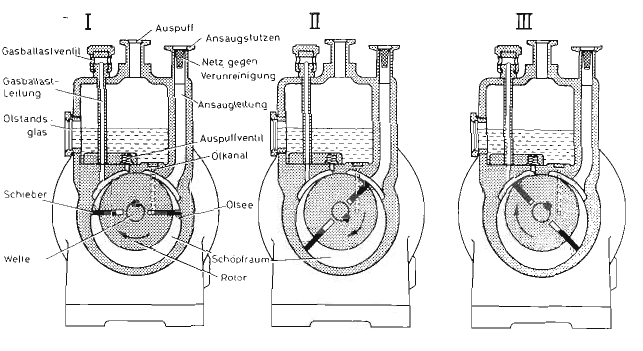
\includegraphics[scale=0.7]{./fig/massenspek_drehschieber.png}
 \caption{Skizze einer Drehschieberpumpe in verschiedenen Zuständen des Pumpvorgangs. Links: Abtrennen des Schöfvolumens. Mitte: Ausstoßen des Gases. Rechts: Ansaugvorgang (Quelle: \cite[S. 7]{Litmap})}
 \label{fig011}
\end{figure}

\subsection{Turbomolekularpumpe}

Eine Turbomolekularpumpe besteht aus einer Statoreinheit und einer Rotoreinheit. Die Rotoreinheit besteht aus einzelnen Schaufeln, die unter einem Winkel $\alpha$ gegen die Diffusionsrichtung gestellt sind.
Die Schaufeln rotieren mit einer Geschwindigkeit $u$, die (am äußeren Rand) ungefähr der mittleren thermischen Geschwindigkeit der Gasmoleküle entspricht. Durch die wiederholte Kollision der Gasmoleküle mit den Rotorschaufeln erhalten diese einen Impuls in Pumprichtung.
Oft sind Turbomolekularpumpen auch aus mehreren hintereinander geschalteten Pumpstufen aufgebaut.

\section{Quadrupol-Massenspektrometer}

In diesem Versuch wird ein Quadrupol-Massenspektrometer (s. Abb. \ref{fig021}) verwendet. Es besteht aus vier hyperbelförmigen Elektroden. Diese erzeugen eine Überlagerung aus einem Gleichfeld $\phi_{1}=U$, das zwischen zwei der Elektroden erzeugt wird, und einem Wechselfeld $\phi_{2}=V\cos(\omega t)$ zwischen den anderen beiden Elektroden.
Die Ionen werden so zwischen den Elektroden auf eine Wellenbahn gezwungen. Das Verhältnis $\frac{U}{V}$ lässt sich so einstellen, dass nur Ionen, die ein bestimmtes Verhältnis $\frac{m}{q}$ der Masse $m$ zur Ladung $q$ besitzen, die Elektroden passieren. Ionen einer anderen Masse stoßen an die Elektroden, und können den Filter nicht passieren.

\begin{figure}[tb]
 \centering
 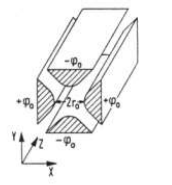
\includegraphics[scale=0.9]{./fig/massenspek_quadrupol.png}
 \caption{Schematische Skizze eines Quadrupol-Massenfilters (Quelle: \cite[S. 25]{Litmap})}
 \label{fig021}
\end{figure}

\section{Ionisationsvakuummeter}

Ein Ionisationsvakuummeter ist ein Messgerät, dass zur Messung niedriger Drücke (im Bereich $10^{-2}$ bis $\SI{e-11}{\milli\bar}$) eingesetzt wird. Zur Messung des Druckes wird mittels einer Glühkathode ein Elektronenstrom erzeugt. Dieser wird über eine Strecke $\Delta l$ durch das Gas zu einem Ionenfänger geleitet.
Die Elektronen stoßen dabei mit den Gasteilchen zusammen und ionisieren diese. Für den dadurch auftretenden Ionenstrom $I^{+}$ gilt
\begin{equation}
 I^{+} = I^{-}S\Delta l,
\end{equation}
mit dem Elektronenstrom $I^{-}$ und der differentiellen Ionisierung $S=n\sigma$, wobei $n$ die Teilchenzahldichte der Gasteilchen und $\sigma$ den Wirkungsquerschnitt des Stoßes bezeichnen.
Für den Zusammenhang von $I^{+}$ mit dem Gasdruck $p$ ergibt sich
\begin{equation}
 I^{+} = \varepsilon I^{-}p,
\end{equation}
mit einer Konstanten $\varepsilon$, die von der Geometrie des Messgeräts abhängt.

\section{Ionenquellen}

Zur Untersuchung der Moleküle ist es notwendig, diese zu ionisieren. Dies kann mit Hilfe folgender Methoden erreicht werden.
\begin{itemize}
 \item Stoßionisation: Diese Methode wird im Versuch verwendet. Hierbei werden die Gasmoleküle mit Elektronen beschossen. Beim Stoß der Elektronen mit den Gasmolekülen kann es zur Ionisation kommen.
 Außerdem kann es zur Dissoziation eines Moleküls kommen, falls die kinetische Energie der Elektronen ausreicht.
 \item Thermische Oberflächenionisation: Von einer heißen Metalloberfläche dampfen adsorbierte Moleküle mit hoher Wahrscheinlichkeit als Ionen ab.
 \item Feldionisation: Hierbei werden die Moleküle in ein stark inhomogenes elektrisches Feld gebracht. Durch den quantenmechanischen Tunneleffekt kann es dabei zur Ionisation kommen.
\end{itemize}


\section{Versuch 1: Einführung}

In diesem Versuch wird zunächst ein Restgasspektrum unter Standardbedingungen ($E=\SI{65}{\electronvolt}, \, I^{-}=\SI{1}{\milli\ampere}$) aufgenommen. Der Versuchsaufbau ist in Abb. \ref{fig0v11} dargestellt.
Es werden Linien bei $m=28,\, 32$ und $44$ erwartet. Diese gehören  zu $\textrm{N}_{2}, \, \textrm{O}_{2}$ und $\textrm{CO}_{2}$.

Für eine Linie wird die Abhängigkeit des Ionenstroms $I^{+}$ vom Elektronenstrom $I^{-}$ gemessen. Es wird erwartet, dass der Ionenstrom mit steigendem Elektronenstrom ansteigt.

\begin{figure}[tb]
 \centering
 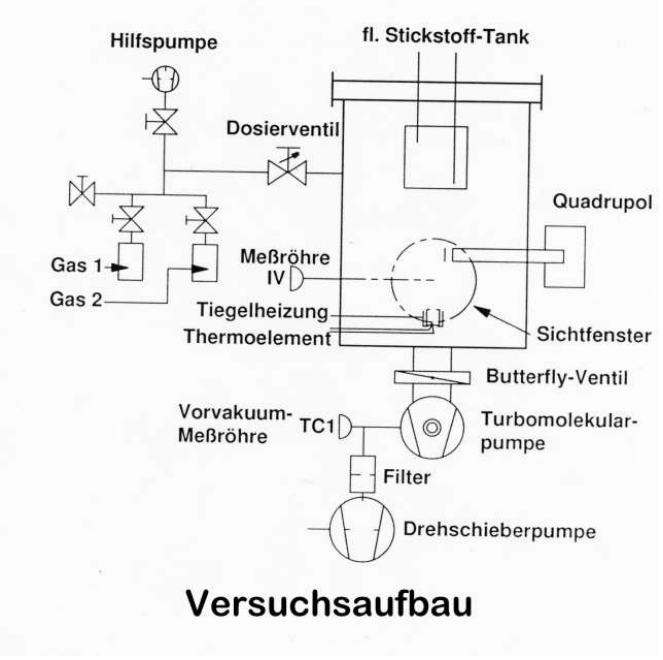
\includegraphics[scale=0.5]{./fig/massenspek_aufbau.png}
 \caption{Schematische Skizze des Versuchsaufbaus (Quelle: \cite[S. 4]{Litmap})}
 \label{fig0v11}
\end{figure}

\section{Versuch 2: Auftrittsenergie von Argon}

In diesem Versuch werden die Auftrittsenergien von Ar$^{+}$ und Ar$^{2+}$ gemessen. Bei der Auftrittsenergie handelt es sich um die Energie der stoßenden Elektronen, ab der die Ionisierung stattfindet.
Dazu wird Argon mit dem Dosierventil bei angeschlossener Turbomolekularpumpe bis zu einem Maximaldruck von $\SI{5e-6}{\milli\bar}$ in den Rezipienten geleitet. Es werden Linien bei $m=40$ (Ar$^{+}$) und $m=20$ (Ar$^{2+}$) erwartet. Dies liegt daran, dass nicht direkt die Massen, sondern das Verhältnis $\frac{q}{m}$ gemessen wird, was bei Ar$^{2+}$ Ionen zu einer scheinbar halb so großen Masse führt.

\section{Versuch 6: Restgasanalyse}

In diesem Versuch wird erneut eine Massenspektrum aufgenommen und daraus quantitativ die Bestandteile des Restgases in der Ionisationskammer bestimmt.
Nachdem die Kammer auf 77\;K herunter gekühlt wurde, wird erwartet, dass die Summe der Partialdrücke geringer als bei Raumtemperatur ist, da zB Wasserdampf bei solch niedrigen Temperaturen fest wird und somit nicht mehr als einzelne Ionen am Detektor gemessen werden kann.

